\documentclass[english,serif,mathserif,xcolor=pdftex,dvipsnames,table]{beamer}
\usetheme{gc3}

\usepackage[T1]{fontenc}
\usepackage[utf8]{inputenc}
\usepackage{babel}

\usepackage{gc3}

\title[Advanced workflows]{%
  More on workflows
}
\author[R. Murri, S3IT UZH]{%
  Riccardo Murri \texttt{<riccardo.murri@uzh.ch>}
  \\[1ex]
  \emph{S3IT: Services and Support for Science IT}
  \\[1ex]
  University of Zurich
}
\date{July~11--14, 2016}

\begin{document}

% title frame
\maketitle


\begin{frame}[fragile]
  \frametitle{Automatic arrangement of tasks}

  Want to avoid arranging tasks in parallel- and sequential- task collections?
  Use a \texttt{DepedentTaskCollection}!

  \+
\begin{python}
from gc3libs.workflow \
  import DependentTaskCollection

class MyWorkflow~\HL{(DependentTaskCollection)}~:
  # ...
  def __init__(self, ...):
    DependentTaskCollection.__init__(self)
    app1 = AnApp(...)
    app2 = AnotherApp(...)
    app3 = AThirdApp(...)
    self.add(app1)
    self.add(app2)
    self.add(app3, after=[app1, app2])
\end{python}
\end{frame}


\begin{frame}[fragile]
  \frametitle{Usage of DependentTaskCollection}

\begin{python}
from gc3libs.workflow \
  import DependentTaskCollection

class MyWorkflow(DependentTaskCollection):
  # ...
  def __init__(self, ...):
    ~\HL{DependentTaskCollection.\_\_init\_\_(self)}~
    app1 = AnApp(...)
    app2 = AnotherApp(...)
    app3 = AThirdApp(...)
    self.add(app1)
    self.add(app2)
    self.add(app3, after=[app1, app2])
\end{python}

  \+
  Initialize the base class.
\end{frame}

\begin{frame}[fragile]
  \frametitle{Usage of DependentTaskCollection}

\begin{python}
from gc3libs.workflow \
  import DependentTaskCollection

class MyWorkflow(DependentTaskCollection):
  # ...
  def __init__(self, ...):
    DependentTaskCollection.__init__(self)
    ~\HL{app1 = AnApp(...)}~
    ~\HL{app2 = AnotherApp(...)}~
    ~\HL{app3 = AThirdApp(...)}~
    self.add(app1)
    self.add(app2)
    self.add(app3, after=[app1, app2])
\end{python}

  \+
  \ldots then initialize tasks that you want to run \ldots
\end{frame}


\begin{frame}[fragile]
  \frametitle{Usage of DependentTaskCollection}

\begin{python}
from gc3libs.workflow \
  import DependentTaskCollection

class MyWorkflow(DependentTaskCollection):
  # ...
  def __init__(self, ...):
    DependentTaskCollection.__init__(self)
    app1 = AnApp(...)
    app2 = AnotherApp(...)
    app3 = AThirdApp(...)
    ~\HL{self.add(app1)}~
    ~\HL{self.add(app2)}~
    ~\HL{self.add(app3, after=[app1, app2])}~
\end{python}

  \+
  \ldots then add tasks to the collection, one by one\ldots
\end{frame}


\begin{frame}[fragile]
  \frametitle{Usage of DependentTaskCollection}

\begin{python}
from gc3libs.workflow \
  import DependentTaskCollection

class MyWorkflow(DependentTaskCollection):
  # ...
  def __init__(self, ...):
    DependentTaskCollection.__init__(self)
    app1 = AnApp(...)
    app2 = AnotherApp(...)
    app3 = AThirdApp(...)
    self.add(app1)
    self.add(app2)
    self.add(app3, ~\HL{after=[app1, app2]}~)
\end{python}

  \+
  \ldots specifying dependencies among them.
\end{frame}


  \begin{frame}
    \frametitle{The \emph{3n+1} conjecture, a fictitious use case}
    \label{sec:7a}

    \+
    \begin{columns}[c]
      \column{0.5\linewidth}
      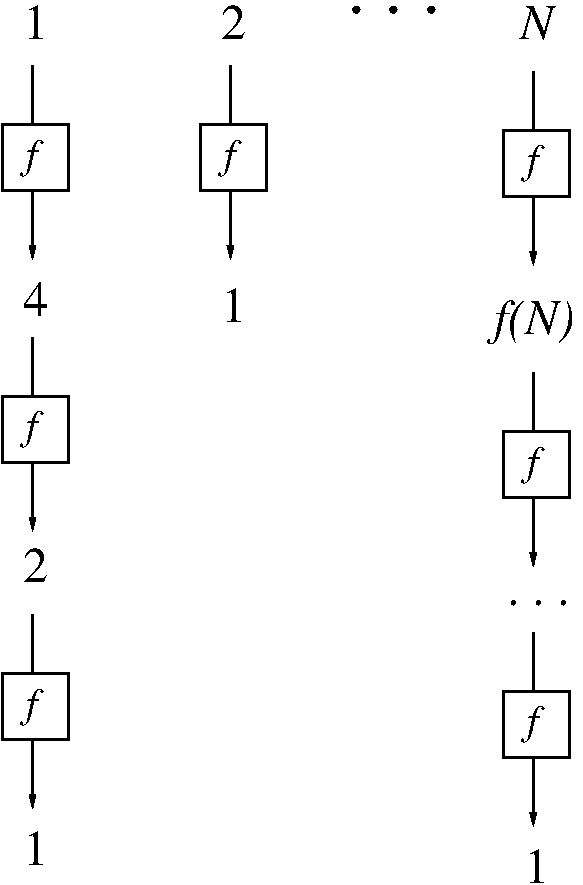
\includegraphics[height=0.8\textheight]{fig/3n+1}

      \column{0.5\linewidth}
      Define a function $f$, for $n$ positive integer:
      \begin{itemize}
      \item if $n$ is even, then $f(n) = n / 2$,
      \item if $n$ is odd, then $f(n) = 3n+1$,
      \end{itemize}

      \+
      For every positive integer $n$, form the sequence $S(n)$:
      $n \to f(n) \to f(f(n)) \to f(f(f(n))) \to \ldots$

      \+
      \textbf{Conjecture:} For every positive integer $n$, the sequence $S(n)$
      eventually hits $1$.
    \end{columns}
  \end{frame}

  \begin{frame}
    \frametitle{The \emph{3n+1} conjecture, \emph{(I)}}
    \label{sec:7}

    \+
    \begin{columns}[c]
      \column{0.5\linewidth}
      \includegraphics[height=0.8\textheight]{fig/3n+1_A}

      \column{0.5\linewidth}
      A computational job $J(n,k)$, applies
      function $f$ to the result of $J(n,k)$.
    \end{columns}
  \end{frame}

  \begin{frame}
    \frametitle{The \emph{3n+1} conjecture, \emph{(II)}}
    \label{sec:7b}

    \+
    \begin{columns}[c]
      \column{0.5\linewidth}
      \includegraphics[height=0.8\textheight]{fig/3n+1_S}

      \column{0.5\linewidth}
      A sequence $H(n)$ of jobs computes the chain $n \to f(n) \to
      ... \to 1$.
    \end{columns}
  \end{frame}

  \begin{frame}
    \frametitle{The \emph{3n+1} conjecture, \emph{(III)}}
    \label{sec:7c}

    \+
    \begin{columns}[c]
      \column{0.5\linewidth}
      \includegraphics[height=0.8\textheight]{fig/3n+1_P}

      \column{0.5\linewidth}
      Run one sequence $H(n)$ per each $n = 1, \ldots, N$.

      \+
      The can all run in \textbf{parallel}.
    \end{columns}
  \end{frame}

\begin{frame}[fragile]
\frametitle{The \emph{3n+1} conjecture (IV)}
\label{sec:10}

\begin{columns}
  \column{0.3\linewidth}
  \begin{center}
    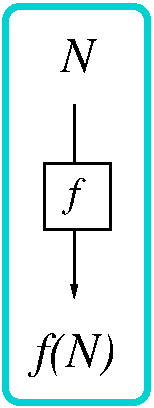
\includegraphics[height=0.8\textheight]{fig/A}
  \end{center}

  \column{0.7\linewidth}
  Let's define the simple application that computes~$f$:
\begin{lstlisting}
class HotpoApplication(Application):
  def __init__(self, n):
    Application.__init__(
      self,
      executable = '/usr/bin/expr',
      arguments = (
          # run `expr n / 2` if n is even
          [n, '/', n] if n % 2 == 0
          # run `expr 1 + 3 * n` if n is odd
          else [1, '+', 3, '*', n]),
      stdout = "stdout.txt",
    )
\end{lstlisting}
  \end{columns}
\end{frame}

\begin{frame}[fragile]
\frametitle{The \emph{3n+1} conjecture (V)}
\label{sec:14}

\begin{columns}
  \column{0.2\linewidth}
  \begin{center}
    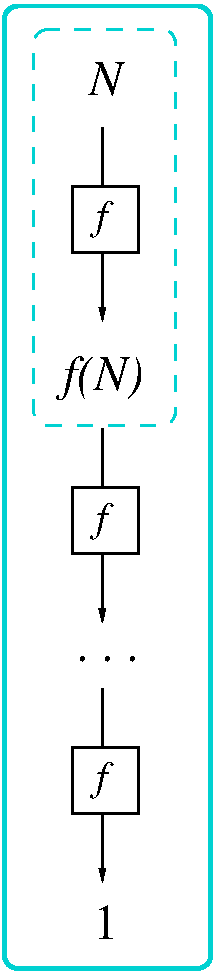
\includegraphics[height=0.8\textheight]{fig/S}
  \end{center}

  \column{0.8\linewidth}
  Now string together applications to compute a
  single sequence:
\begin{lstlisting}
class HotpoSequence(SequentialTask):

  def __init__(self, n):
    # compute first iteration of $f$
    self.tasks = [ HotpoApplication(n) ]
    SequentialTask.__init__(self, self.tasks)

  def next(self, k):
    last = self.tasks[k].result
    if last == 1:
      return TERMINATED
    else:
      self.tasks.append(MyApplication(last)
       return RUNNING
\end{lstlisting}
  \end{columns}
\end{frame}

\begin{frame}[fragile]
  \frametitle{The \emph{3n+1} conjecture (VI)}
  \label{sec:15}

  \begin{columns}
    \column{0.5\linewidth}
    \begin{center}
      \includegraphics[height=0.8\textheight]{fig/3n+1_P}
    \end{center}

    \column{0.5\linewidth}
    Parallel tasks are independent by definition, so it's even easier to
    create a collection:
\begin{lstlisting}
tasks =
  ParallelTaskCollection([
    HotpoSequence(n)
      for n in range(1, N) ])
\end{lstlisting}

    We can run such a collection like any other \texttt{Task}.
  \end{columns}
\end{frame}

\end{document}

%%% Local Variables:
%%% mode: latex
%%% TeX-master: t
%%% End:
